\begin{figure}[h!]
     \centering
    \captionsetup[sub]{font=small}
     \begin{subfigure}[b!]{0.3 \textwidth}
         \caption{}
         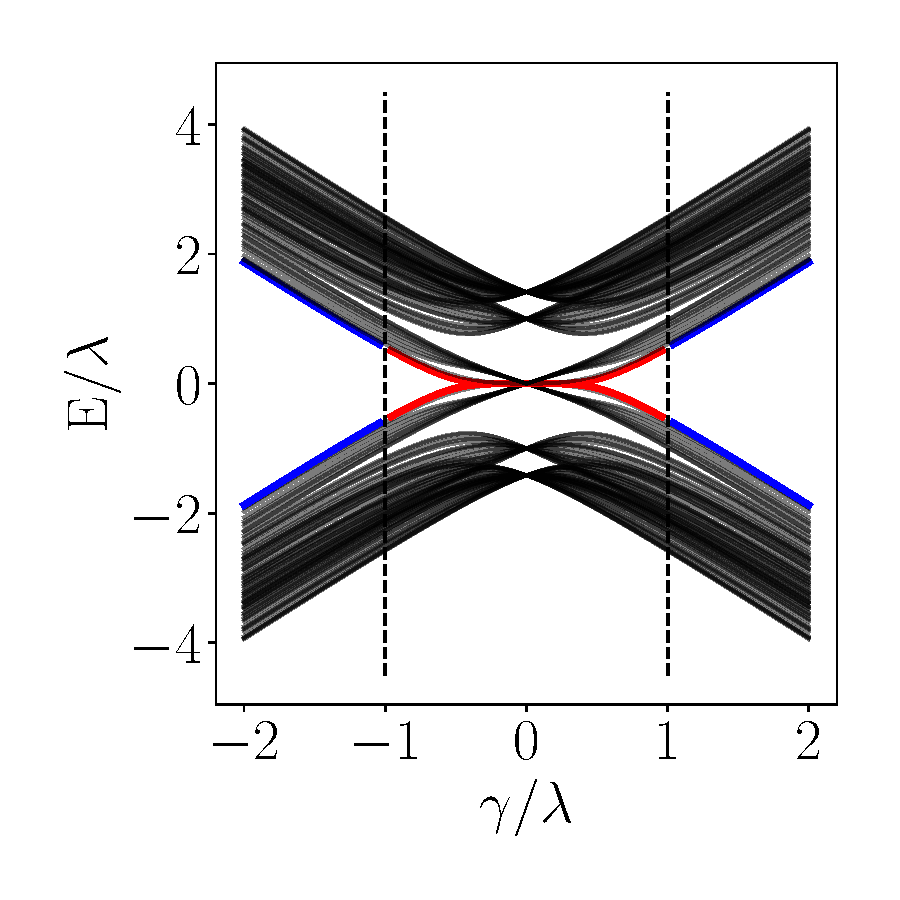
\includegraphics[width=\textwidth]{Imagenes/Resultados_Hoti_Fractal/bands_square_shh.pdf}
         \label{}
     \end{subfigure}\hspace*{-0.5em}
     \begin{subfigure}[b!]{0.3 \textwidth}
         \caption{}
         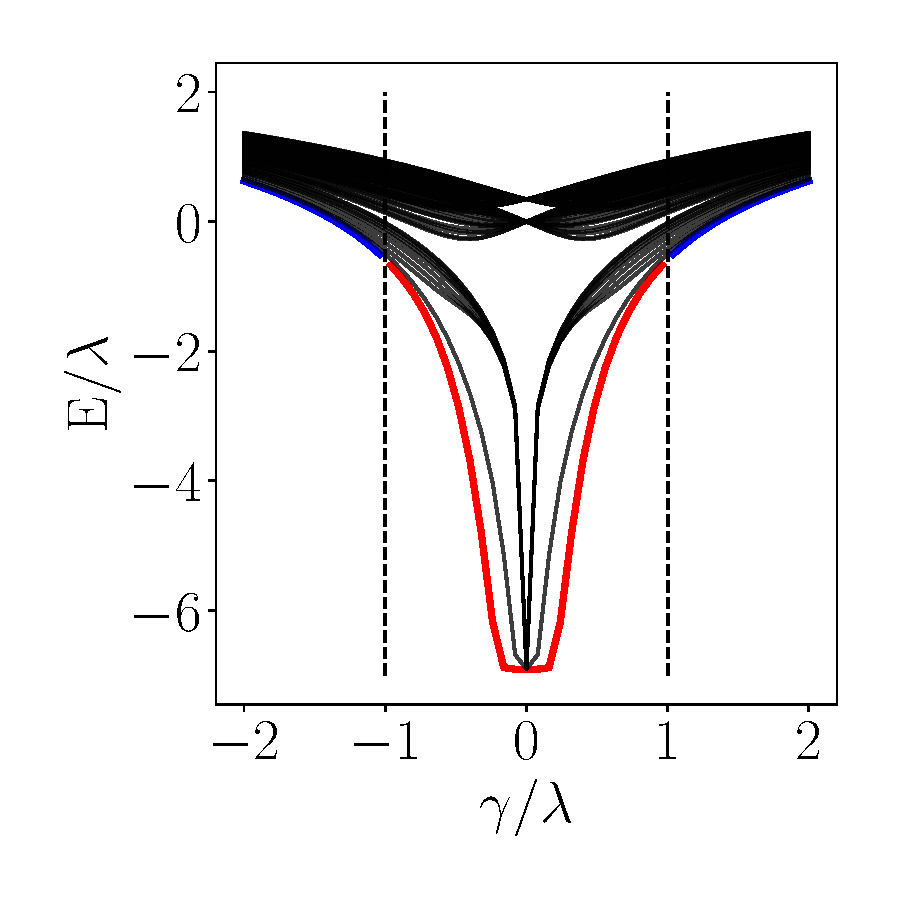
\includegraphics[width=\textwidth]{Imagenes/Resultados_Hoti_Fractal/bands_square_shh_log.pdf}
         \label{}
     \end{subfigure}\hspace*{-0.5em} 
      \begin{subfigure}[b!]{0.4 \textwidth}
         \caption{}
         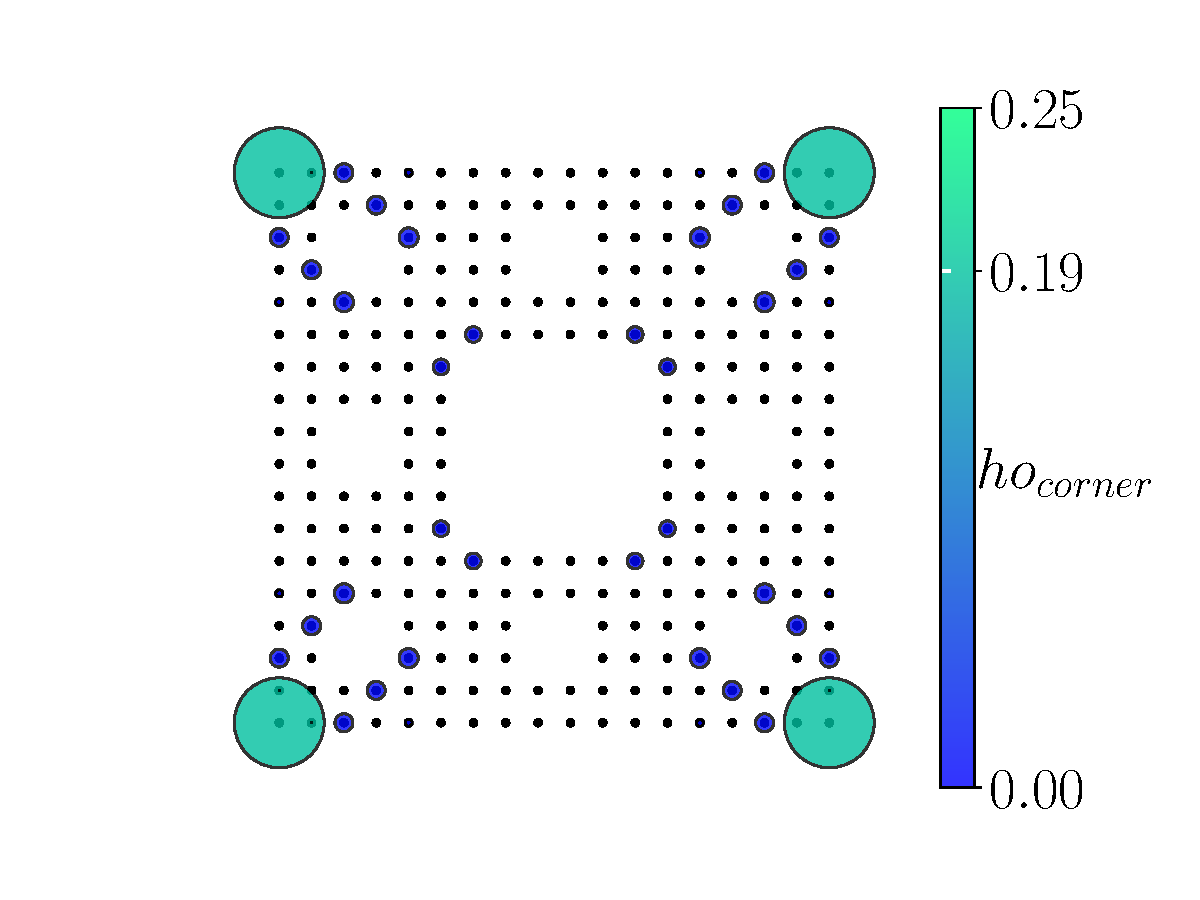
\includegraphics[width=\textwidth]{Imagenes/Resultados_Hoti_Fractal/proyection_square.pdf}
         \label{}
     \end{subfigure}\hspace*{-0.5em} \vspace*{-1.5em}
        \caption{\textbf{a)} Espectro de energía del sistema con geometría fractal y condiciones abiertas a la frontera, como función de $\gamma/\lambda$. \textbf{b)} Espectro de energía en escala logarítmica del sistema antes mencionado. Las lineas rojas corresponden a los cuatro estados degenerados que representan los estados localizados en las esquinas. \textbf{b)} Densidad de probabilidad en un fase no trivial donde $\gamma = 1,\, \, \lambda = 4.5$, en un red fractal de 2da generación.}
\label{fig:Param_Proy_fractal}
\end{figure}